\subsubsection{Batch Uniformisation}

First of all we chose one of the selected approaches (NNs, SVMs or
LWPR) and one problem (classification or regression) for initial
experimentation. We decided to use SVMs for classification. so far,
the data were retained in full, with no subsampling. We then decided,
as a start, to test whether data obtained during one session could be
used to build a model able to generalise over other sessions during
the same day.

Here an obvious problem arises: the total time of the experiment
during which data were gathered was about $100$ minutes; at $256$Hz,
that means about $1.6$ millions samples, an unfeasibly large training
set for any of the examined methods, not to mention SVM
classification. Even restricting a training set to a single session,
this would result in about $53000$ samples, which not only is still
too large, but probably contains redundant and irrelevant information.
Moreover, in a real setting, this number is doomed to grow continually
and cannot therefore be used as it is for periodical re-training. We
then decided to investigate a smart sample reduction strategy in order
both to overcome this problem, but also to gain insight into the EMG
signal in general. This led us to develop the batch version of the
uniformisation procedure.

The simple idea behind batch uniformisation is that, in a real-life
set-up such as ours, there can be many input samples located in the
very same region of the input space, with very similar target
values. One obvious case is that of label $0$, indicating no ongoing
grasping: it is intuitively expected that a large number of samples
will be taken in that region of the input space, since the subject
will be in the $0$ condition for a longer time than all other
labels. Since all functions involved in the experiment are due to
human motion, we can assume that they are continuous and, probably,
derivable up to any arbitrary order. Therefore it makes no sense to
consider samples obtained in a non-uniform way such as that described
above. The batch uniformisation procedure consists of removing, from a
training set, those samples which are \emph{too close to each other},
according to a suitable notion of inter-sample distance.

In order to take into account the variance of each single electrode,
and since in batch data analysis all data are available beforehand and
therefore all possible statistics can be gathered a-priori, we have
decided to adopt Mahalanobis's distance as the inter-sample
distance. Let $\xx_1, \xx_2 \in \RR^{10}$; then the Mahalanobis
distance between $\xx_1$ and $\xx_2$ is defined as follows:

$$ MD(\xx_1,\xx_2) = \sqrt{(\xx_1-\xx_2)^T \Sigma^{-1} (\xx_1-\xx_2)} $$

\noindent where $\Sigma$ is the $10$x$10$ covariance matrix, evaluated
on the whole training set. $MD(\xx_1,\xx_2)$ is a measure of distance
independent of the (co)variance of the electrodes. (Notice that if
$\Sigma$ is replaced by the identity matrix, $MD(\xx_1,\xx_2)$ is
reduced to the usual notion of Euclidean distance.)

Since checking the inter-sample distance on a batch of samples
obviously takes a quadratic time with respect to the number of
samples, which was unfeasible, we adopted an approximated method which
was able to remove most, but not all, samples too Mahalanobis-close to
each other. After a few initial experiments, the threshold distance
was set at $1$. Notice that no \emph{testing} set was uniformised.
Notice, further, that applying uniformisation resulted in training
sets which were considerably smaller than the original ones, up to
about $100$ times smaller.

The first question is: do uniformised training sets lack any relevant
information? We trained a SVM over each single session, both for the
first and second day, and both with full and uniformised training
sets. The session were numbered chronologically during the day,
sessions $1,2,3$ forming group $1$, sessions $4,5,6$ forming group
$2$, and so on. With a slight abuse of language, we will call the
model obtained by training a machine on session $i$, \emph{model
$i$}. Moreover, in the remainder of this Subsection, if the training
set of a model was uniformised, we will call the model \emph{uniform}.

We then tested each model on all sessions of the same day, obtaining
therefore an \emph{accuracy matrix} $A$ in which $A_{ij}$ would be a
percentage denoting the correctly guessed labels when testing model
$i$ (full or uniform) on session $j$. Notice once again that, in the
case of uniform models, the test is carried out on the \emph{full}
session. This is what we would call a \emph{cross-session analysis}.
The result is visible in Figure \ref{fig:cross_initial}.

\begin{figure}[!ht] \centering
  \begin{tabular}{cc}
    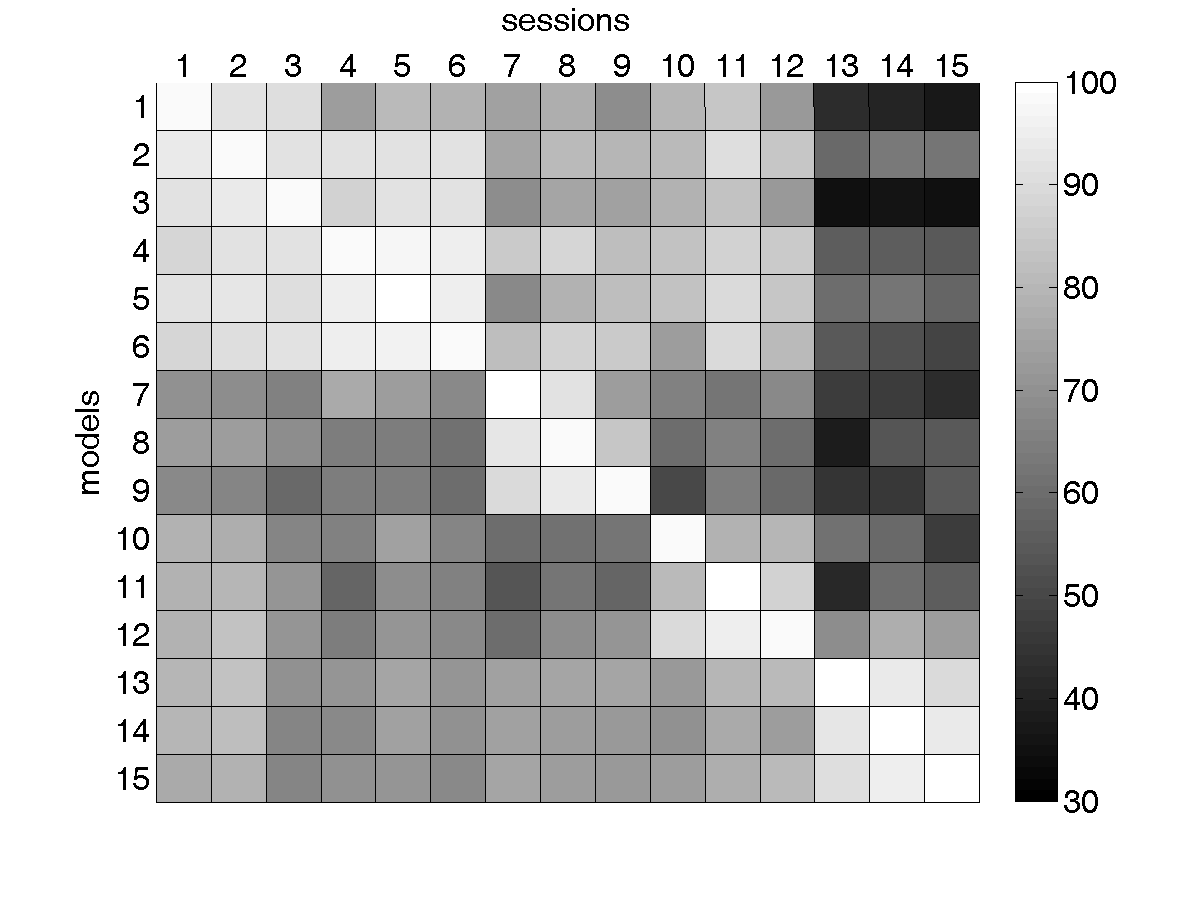
\includegraphics[width=0.22\textwidth]{figs/fig_resCross1_full} &
    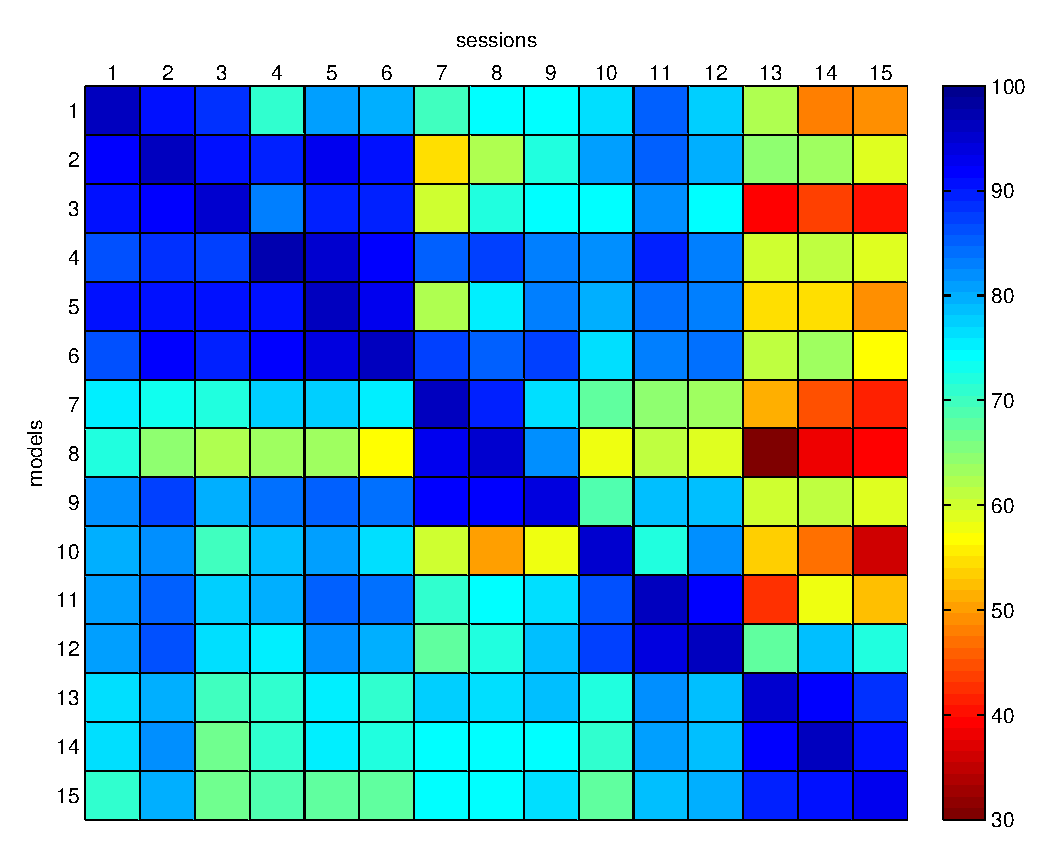
\includegraphics[width=0.22\textwidth]{figs/fig_resCross1} \\
    diagonal: $98.73\% \pm 0.39\%$  & diagonal: $95.52\% \pm 1.21\%$ \\
        rest: $73.23\% \pm 14.29\%$ & rest: $74.53\% \pm 13.70\%$ \\
    $(a)$ & $(b)$ \\
    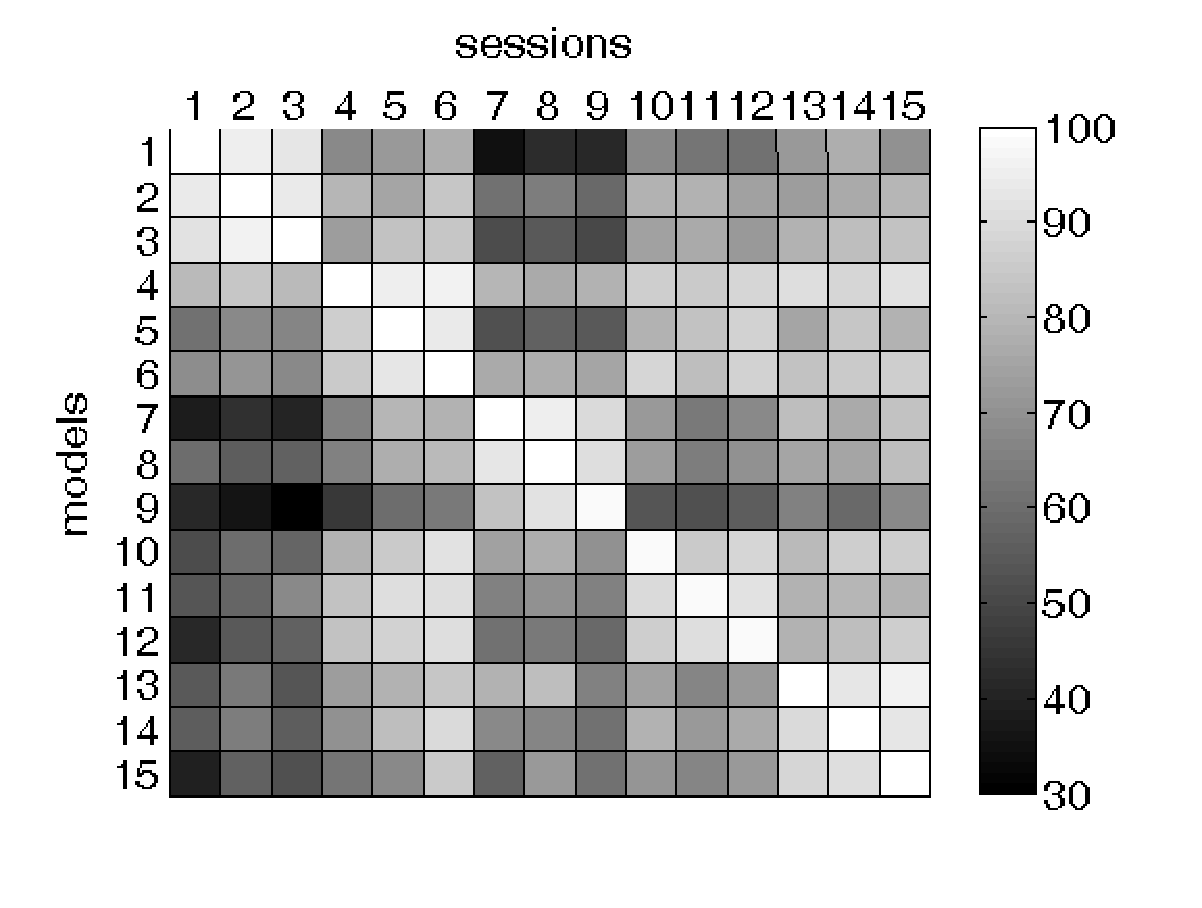
\includegraphics[width=0.22\textwidth]{figs/fig_resCross2_full} &
    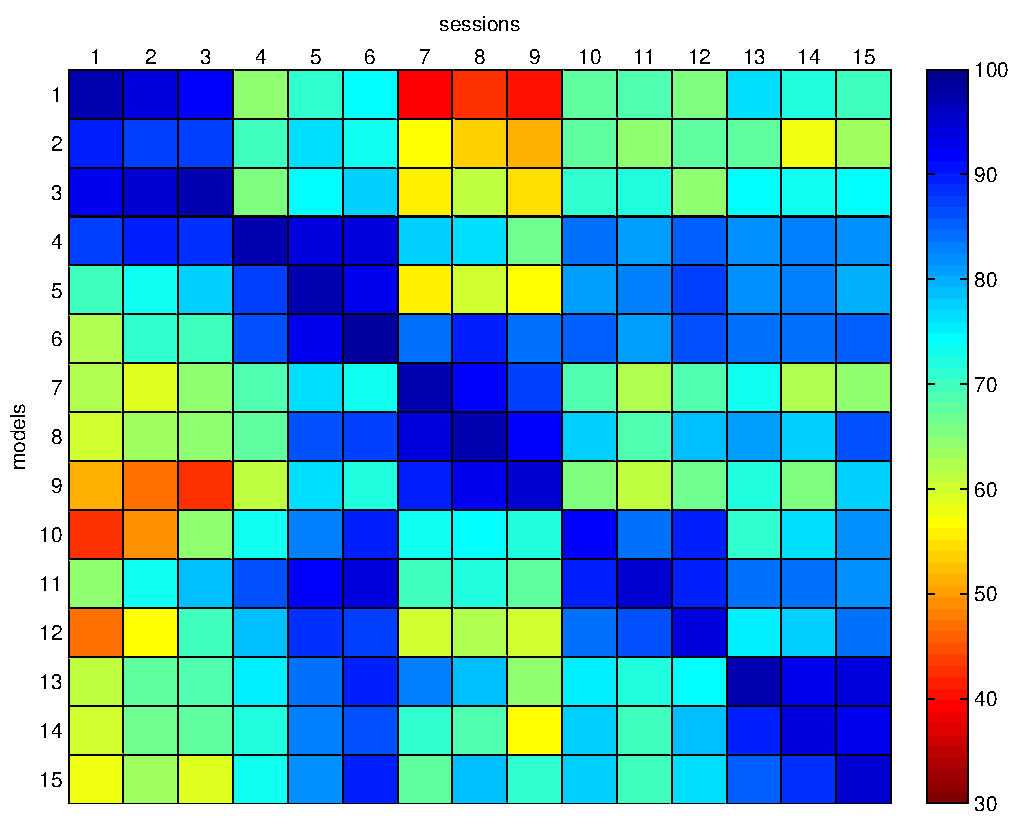
\includegraphics[width=0.22\textwidth]{figs/fig_resCross2} \\
    diagonal: $99.05\% \pm 0.37\%$ & diagonal: $95.37\% \pm 2.85\%$ \\
        rest: $73.23\% \pm 14.47\%$ & rest: $74.38\% \pm 12.27\%$ \\
    $(c)$ & $(d)$ \\
  \end{tabular}
  \caption{Cross-session analysis and evaluation of the uniformisation
    procedure. $(a)$ and $(b)$, accuracy matrices for day $1$: $(a)$
    full models, $(b)$ uniform models. $(c)$ and $(d)$, same for day $2$.}
  \label{fig:cross_initial}
\end{figure}

Consider first panes $(a)$ and $(b)$ of the Figure, pane $(a)$ being
the accuracy matrix for full models, day $1$, and pane $(b)$ being the
accuracy matrix for the same day, but using uniform models. It is
apparent from the colours that the full models attain a better
accuracy when tested on their own training data, that is, on the
diagonal of the matrix, than the uniform models. In fact, the mean and
standard deviation of the diagonal accuracies are $98.73\% \pm 0.39\%$
for the full models and $95.52\% \pm 1.21\%$ for the uniform
models. This is intuitively sensible since, in the case of full
models, we are testing on the same data used for training, whereas in
the case of uniform models, the training data are a strict subset of
the testing data, and a quite smaller subset indeed. But as well, if
we consider the remaining elements of the matrices, it is clear that
the uniform models attain a better accuracy \emph{overall}, if
compared to the full models. In fact, the accuracies are $73.23\% \pm
14.29\%$ for the full models, and $74.53\% \pm 13.70\%$ for the
uniform ones. The same analysis for day $2$ yields analogous results
(consider the above Figure, panes $(c)$ and $(d)$).

From this we conclude that the uniformisation procedure is effective
in reducing the training set size, \emph{without actually degrading
the performance}. This is apparent from the fact that uniform models
are more accurate on testing sets which are disjoint from the training
sets. In fact, one should always ensure that this is the case, aiming
for a better generalisation error. We can say that uniform models
generalise better, at least in this case.

\subsubsection{Classification}

Consider Figure \ref{fig:cross_initial} again, right hand side panes
($(b)$ and $(d)$) and the numbers below. The accuracy attained on
non-diagonal elements is about $74\%$, which is rather bad. One cannot
expect to correctly drive a prosthesis if one sample in four is
misclassified. At the same time, however, a strong ``good group
accuracy'' is obviously present: in each matrix, good accuracy values
are obtained on 3x3 submatrices located on the diagonals,
corresponding to cross-session accuracy for sessions \emph{belonging
to the same group}, that is, where the elastic bands were not removed
and no electrode displacement was present.

More in detail, as far as the first day is concerned (same Figure,
pane $(b)$), one can see that the first six models (trained on the
first two groups) obtain a quite good accuracy on the first six
sessions (first two groups) whereas their accuracy rapidly degrades as
more sessions are tested for. This is probably due to the first two
groups having been gathered in similar conditions, very similar
electrode positions and/or similar movements performed by the
subject. On the other hand, sessions in the last group (columns $13$,
$14$ and $15$ of the matrix) are particularly hard, except when tested
by models obtained from the last group itself --- here the effect is
probably motivated by the opposite reason: during those sessions, the
subject must have explored different parts of the input space. This is
corroborated by the fact that models $13,14,15$ perform rather well on
\emph{all} sessions, if compared to other models (check rows
$13,14,15$ of the matrix). In other words, sessions $13,14,15$ contain
more relevant information than the others.

Analogous considerations can be made by inspecting the accuracy matrix
of the second day, pane $(d)$ of the Figure.

From this we can confirm that \emph{electrode displacement plays a
determinant role} in the classification accuracy. Notice that muscle
fatigue seems not to enter the picture, but this is reasonable since
its effetcs are visible already within one single session (see Figure
\ref{fig:drift} again) and the machine correctly takes it into account
during the training phase. Notice once again that the uniformisation
procedure does not hinder the generalisation power of the system.

It is intuitively expected that the poor cross-session generalisation
performance is due to the problem of electrode displacement. This is
experimentally confirmed by the strong degradation in classification
accuracy among different groups. In other words, the SVM does not
generalise well when trained on a session belonging to group and
tested on a session belonging to a different group. Electrode
displacement present between groups (but not within a group) causes
the samples in a group to be ``shifted'' in the input space, so that
testing on a different group results in poor generalisation
performance. To substantiate this claim, we have verified that the
cross-session accuracy is highly correlated to the \emph{average
minimum inter-sample distance} between sessions. More in detail, let
$S_i$ and $S_j$ denote the sets of samples gathered during sessions
$i$ and $j$; then the \emph{cross-session distance matrix} $D$ is such
that

$$ D_{ij} = \frac{1}{|S_j|} \sum_{s_j \in S_j}{\min_{s_i \in S_i}{ ||s_j-s_i||^2 } } $$

Essentially, $D_{ij}$ denotes how far away in the input space the
samples in $S_j$ are from the samples in $S_i$. Note that $D$ is in
general not symmetric.

The cross-correlation coefficient evaluated between $D$ and the
cross-session accuracy matrix is about $-0.61$ \emph{both} for the
first and the second day, indicating a strong negative correlation.
Further experiments have revealed that this happens for Neural
Networks too (cross-correlation $-0.40$ for day $1$ and $-0.51$ for
day $2$); and also, that $D$ is strongly \emph{positively} correlated
to the MSE in regression, for all the studied approaches: $0.62/0.78$
(day $1$/day $2$) for SVMs, $0.64/0.72$ for NNs and $0.77/0.81$ for
LWPR. In other words, the larger the distance of $S_i$ and $S_j$, the
worse the performance of model $i$ tested on session $j$, \emph{both
in classification and in regression}, and \emph{for all approaches
tested}. This tells us that $(a)$ samples of the same group are closer
to each other than sample from different groups, therefore electrode
displacement causes displacement in the input space too; and $(b)$
that this causes bad inter-group performance. ``Samples far away from
the training set will be predicted badly.''

%% In order to further sustain this claim we have checked, for each day,
%% that models obtained by adjoining $4$ of the $5$ groups would perform
%% well on the group excluded when training; this would indeed indicate
%% that more data is needed to train the machine, and that the required
%% data must somehow be found in some of (but not necessarily all) the
%% gathered groups. We will call these models \emph{multi-group
%% models}. The results are visible in Figure \ref{fig:bigmodels}.

%% \begin{figure*}[!ht] \centering
%%   \begin{tabular}{cc}
%%     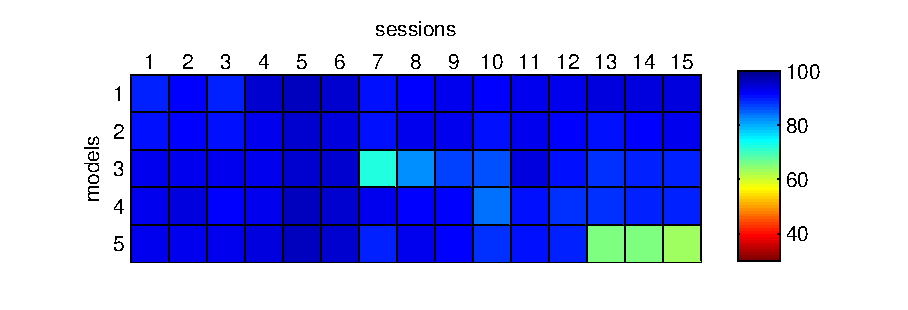
\includegraphics[width=0.45\textwidth]{figs/fig_resCross_day1_big} & 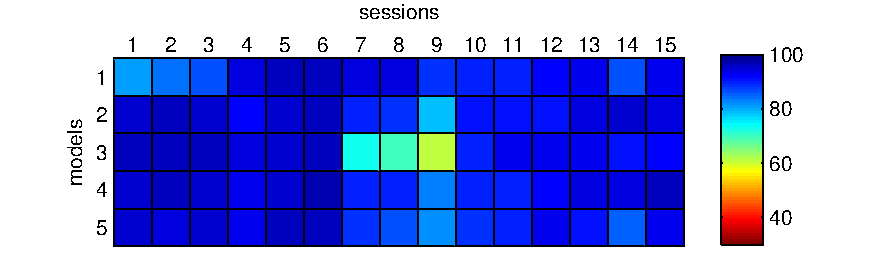
\includegraphics[width=0.45\textwidth]{figs/fig_resCross_day2_big} \\
%%     $(a)$ & $(b)$ \\
%%   \end{tabular}
%%   \caption{Cross-session analysis of multi-group models, obtained by adjoining $4$
%%     of the $5$ groups of each day. Each row denotes the model trained
%%     excluding group $1,\ldots,5$ from the model itself. $(a)$ day $1$, $(b)$ day $2$.}
%%   \label{fig:bigmodels}
%% \end{figure*}

%% Consider the rows of the matrices in the Figure: as one can see, the
%% accuracy is uniformly very high, even when the models are tested on
%% unseen testing data; for instance, model $1$ of day $1$ has an
%% accuracy of $92.82\% \pm 1.96\%$, and model $4$ of day $2$ has an
%% accuracy of $92.64\% \pm 3.73\%$. Moreover, notice that, e.g., model
%% $5$ of day $1$ performs badly on group $5$ of day $1$, as one can
%% expect, since model $5$ has not been trained on that very group, which
%% was already determined to be very hard (compare Figure
%% \ref{fig:cross_initial}, pane $(b)$, last three columns).

%%  Model $1$ of day $1$, for
%% instance, performs uniformly very well. From this we first conclude
%% that the uniformisation procedure is not eliminating any useful
%% information from the training sets; and, secondly, that if the right
%% training data can be found, there are good chances of building a good
%% model.

The dual consideration is that if we train upon the ``right'' data,
the accuracy should become acceptable. How to find the right data
then? In this batch phase, we have deicded to adjoin two models per
day, which would obtain a good accuracy on all sessions. For instance,
consider Figure \ref{fig:cross_initial} again, pane $(b)$. It is
apparent that model $4$ performs well on groups $1$ to $4$, whereas
model $13$ does well on group $5$ (and is not bad on the
others). These two models were used to form a ``best'' training set
which would give good results on the whole day $1$. Analogous
considerations led us to use also models $4$ and $8$ of day $2$. The
obtained model will be called \emph{best} model.

This procedure was repeated for each problem tackled (classification,
regression) and approach tested (SVM, NN and LWPR). Figure
\ref{fig:best_class} shows the classification accuracy of the best
models for classification on all sessions of day $1$ and $2$, for SVMs
and NNs. The analysis detailed in the previous Subsection has been
repeated for the Neural Network. In that case, models $8$ and $15$ of
day $1$, and models $3$ and $10$ of day $2$ have been used to build
the best model.

\begin{figure}[!ht] \centering
  \begin{tabular}{cc}
    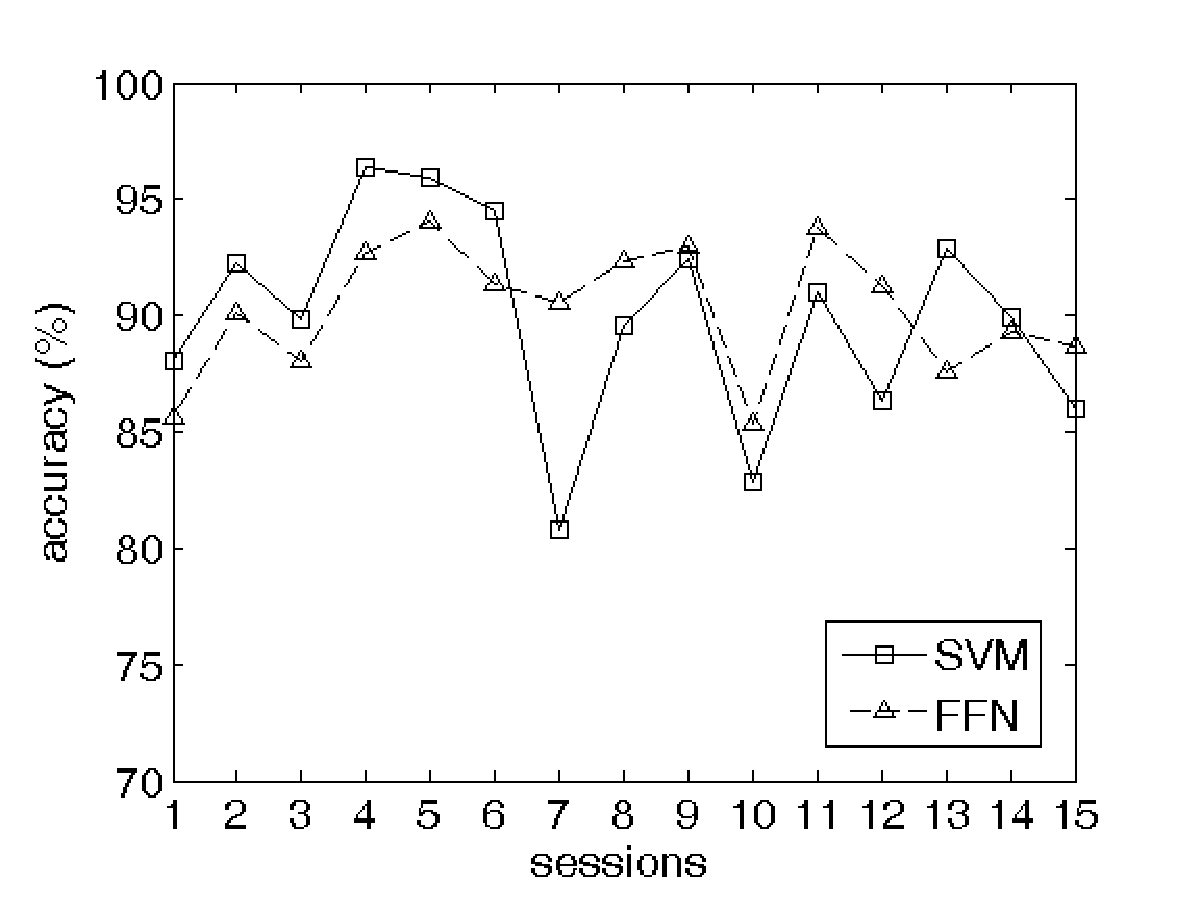
\includegraphics[width=0.22\textwidth]{figs/fig_class_resCrossBestOnDay1} &
    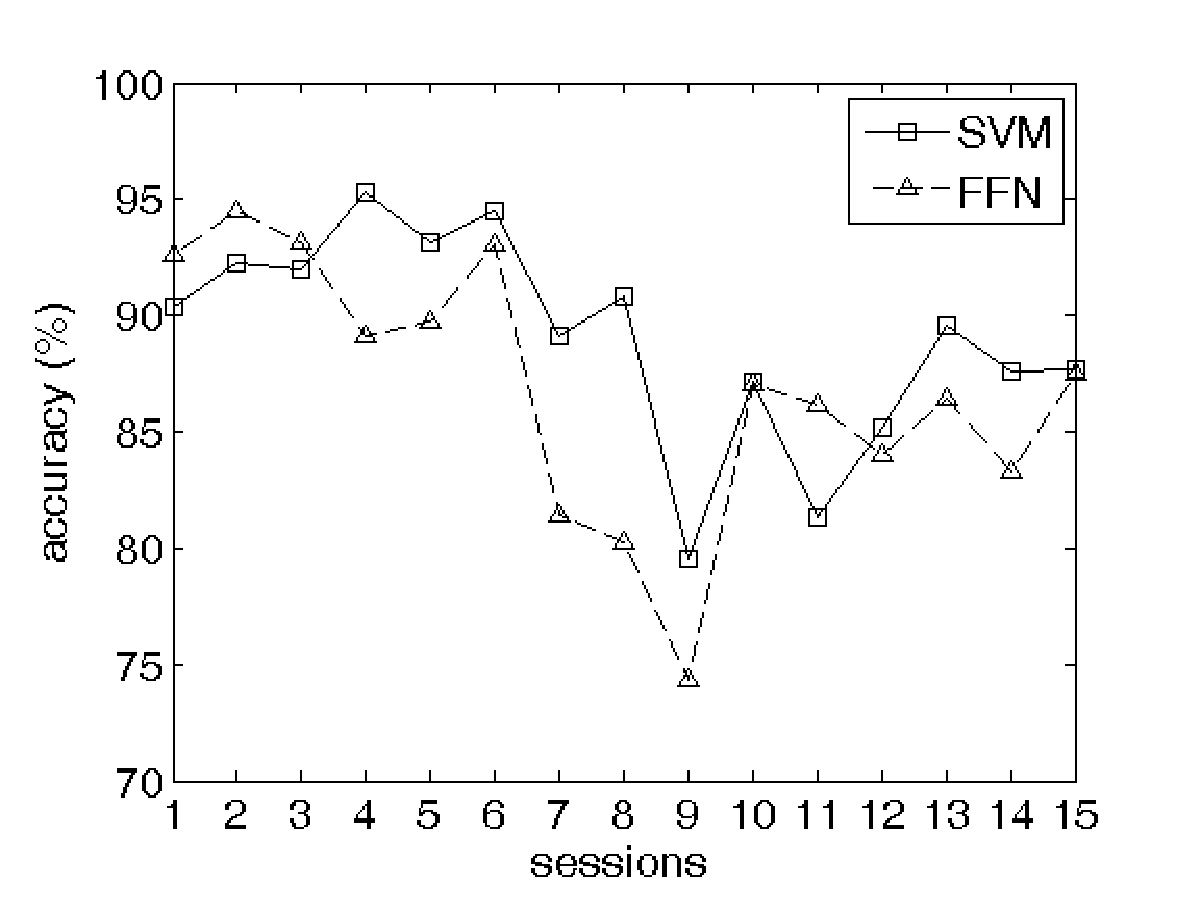
\includegraphics[width=0.22\textwidth]{figs/fig_class_resCrossBestOnDay2} \\
    SVM: $89.90\% \pm 4.51\%$ & SVM: $89.04\% \pm 4.50\%$ \\
     NN: $90.25\% \pm 2.77\%$ &  NN: $86.84\% \pm 5.57\%$ \\
    $(a)$ & $(b)$ \\
  \end{tabular}
  \caption{Classification accuracy of best models, day $1$ $(a)$ and
    day $2$ $(b)$.}
  \label{fig:best_class}
\end{figure}

As one can see, there is no clear winner between SVMs and NNs. NNs
perform slightly better on day $1$ (higher mean, lower standard
deviation) but SVMs are analogously better on day $2$. All in all,
classification accuracy is good, at an overall rate of about
$90\%$. In this case, the training data amounts to four sessions
(uniformised in the case of SVMs and full in the case of NNs), which
is about $12$-$15$ minutes of user activity. But notice, that samples
gathered during both days were necessary to have an idea of which
sessions to use.

\subsubsection{Regression}

Lastly, the most interesting part was how to predict the amount of
force applied by the subject by looking at the EMG signal. To do this,
we have repeated once again the analysis done in Subsection
\ref{subsec:strategy} for the three approaches selected, and found out
that the four sessions involved in the best models were: $6,12,3,12$
for SVMs, $4,11,3,12$ for NNs and $6,13,3,4$ for LWPR. We have
considered three indices of performance: the Mean Squared Error (MSE)
in its standard definition; the Normalised Root MSE (NRMSE), ratio of
the square root of the MSE and the range of the target values,
expressed as a percentage; and the Squared Correlation Coefficient
(SCC) between the predicted target and the real target.

\begin{figure}[!ht] \centering
  \begin{tabular}{cc}
    \includegraphics[width=0.22\textwidth]{figs/fig_err_regr_resCrossBestOnDay1} &
    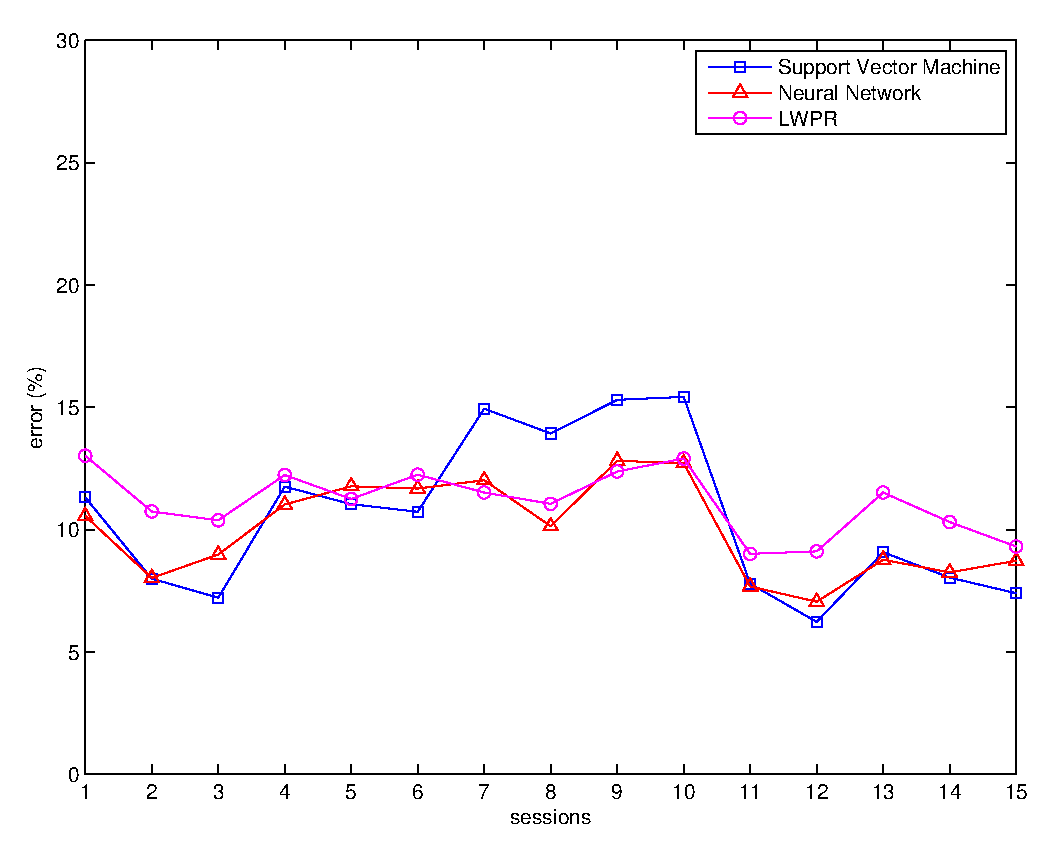
\includegraphics[width=0.22\textwidth]{figs/fig_err_regr_resCrossBestOnDay2} \\
     SVM: $11.84\% \pm 2.64\%$ &  SVM: $10.54\% \pm 3.18\%$ \\
      NN: $10.54\% \pm 1.41\%$ &   NN: $10.01\% \pm 1.93\%$ \\
    LWPR: $11.98\% \pm 1.31\%$ & LWPR: $11.13\% \pm 1.32\%$ \\
    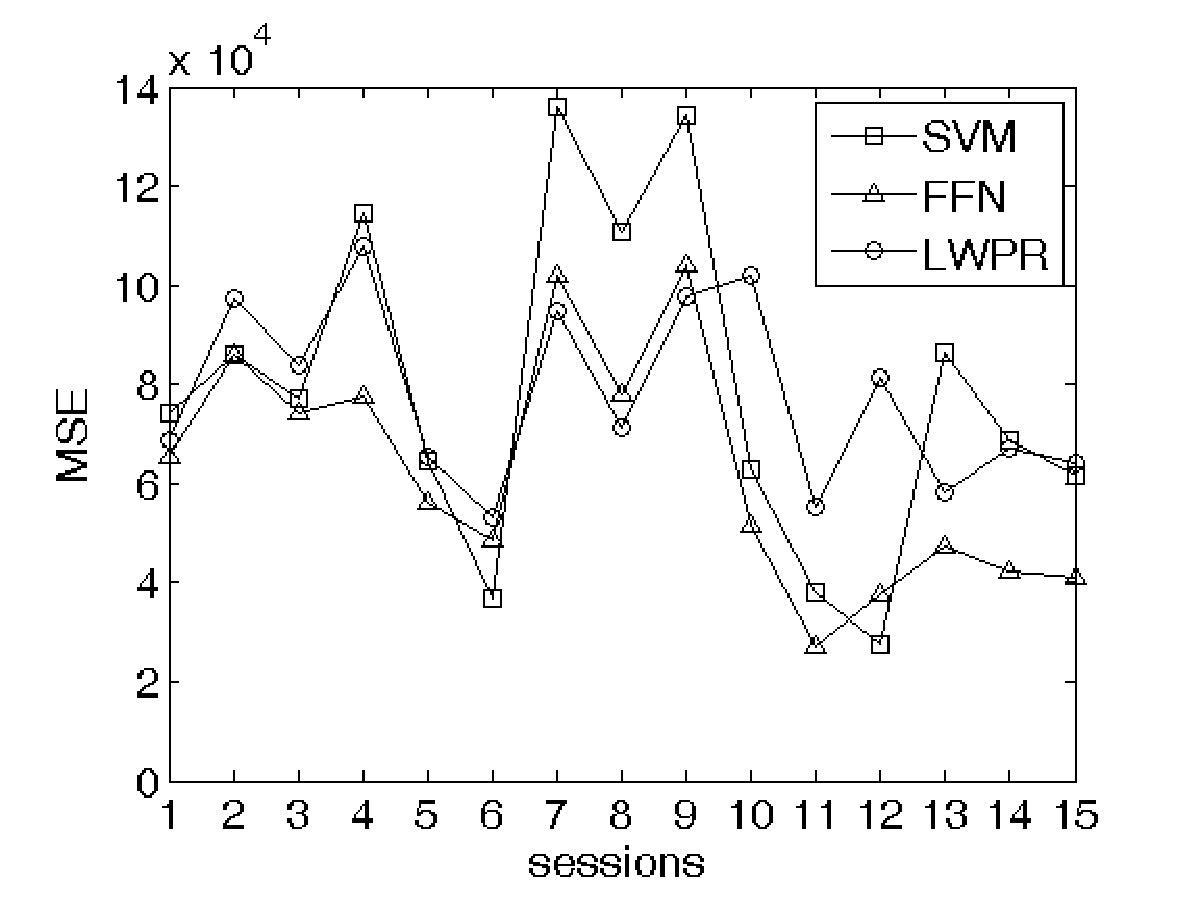
\includegraphics[width=0.22\textwidth]{figs/fig_MSE_regr_resCrossBestOnDay1} &
    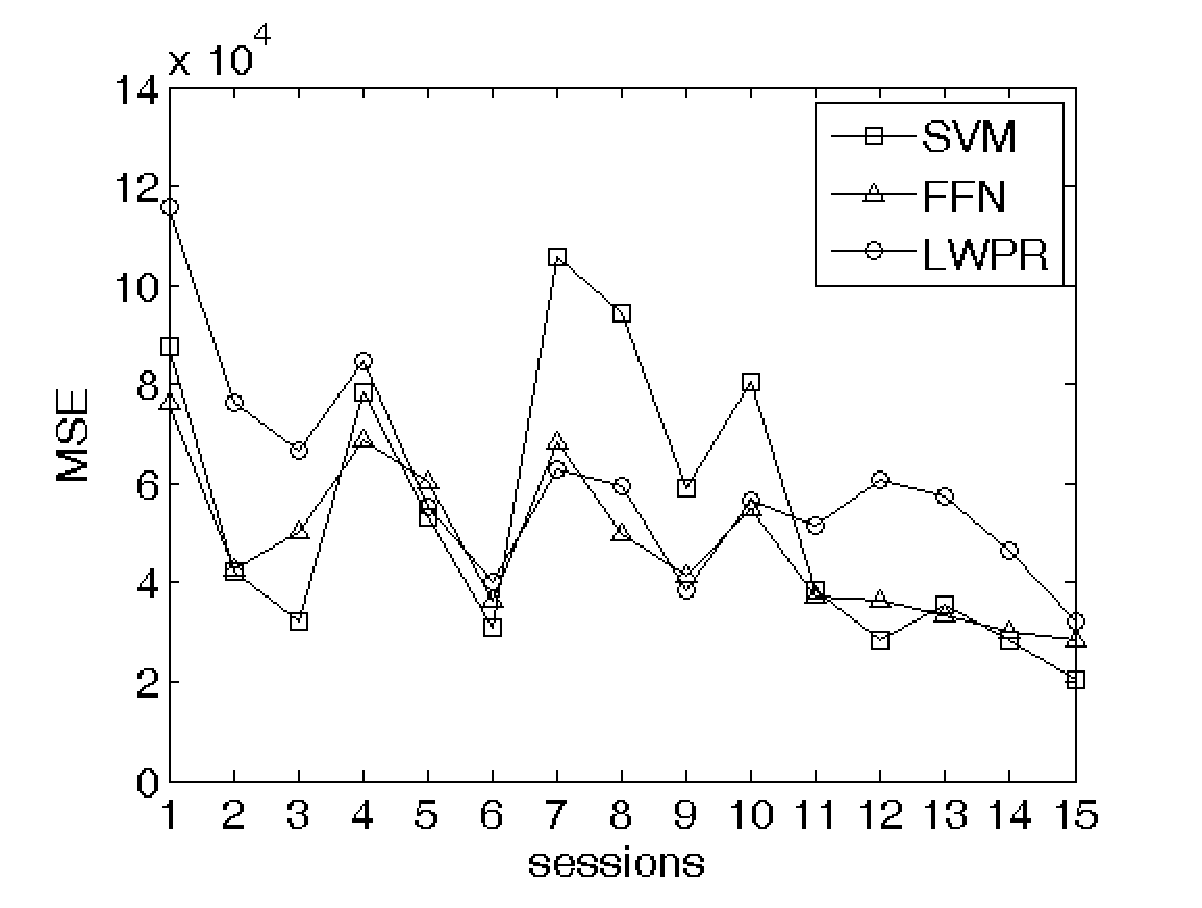
\includegraphics[width=0.22\textwidth]{figs/fig_MSE_regr_resCrossBestOnDay2} \\
     SVM: $7.86 \pm 3.35$ &  SVM: $5.44 \pm 2.79$ \\
      NN: $6.27 \pm 2.36$ &   NN: $4.76 \pm 1.52$ \\
    LWPR: $7.79 \pm 1.83$ & LWPR: $6.03 \pm 2.07$ \\
    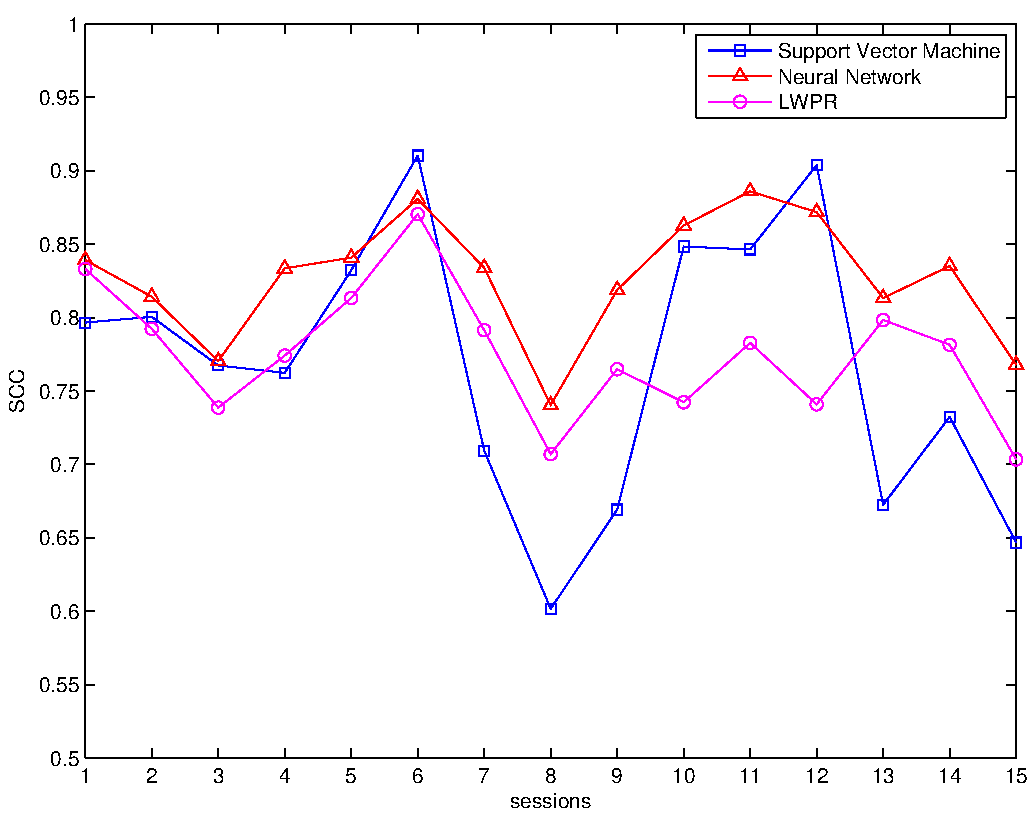
\includegraphics[width=0.22\textwidth]{figs/fig_SCC_regr_resCrossBestOnDay1} &
    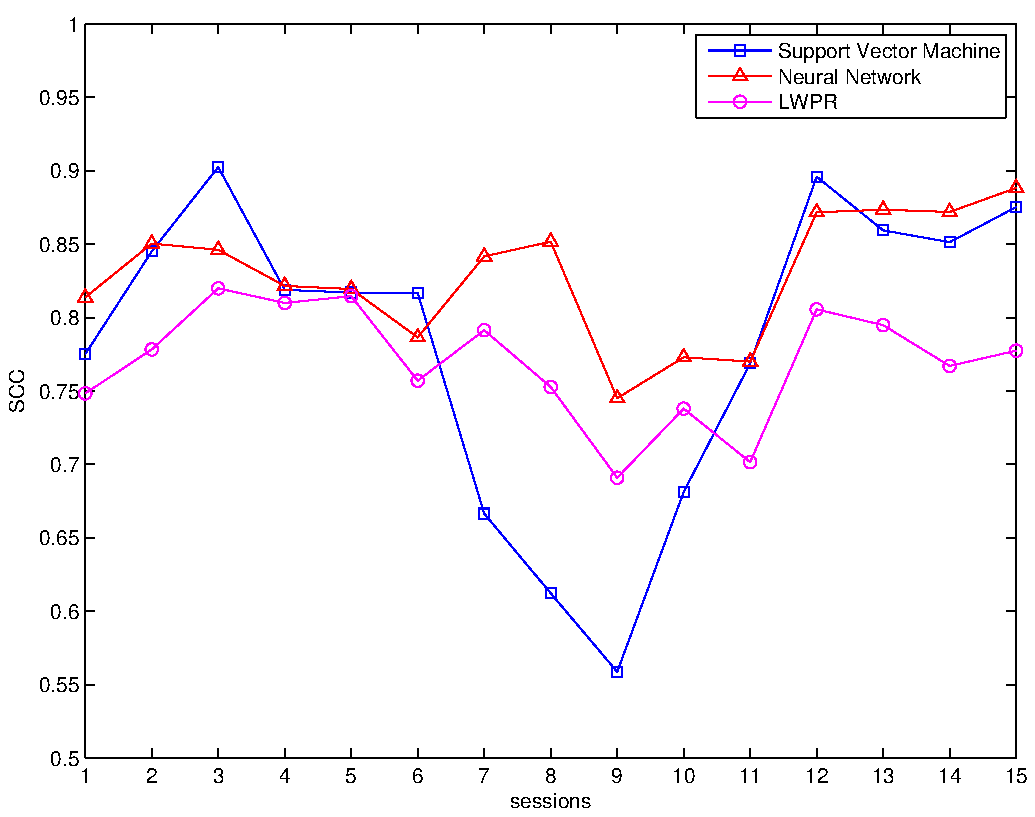
\includegraphics[width=0.22\textwidth]{figs/fig_SCC_regr_resCrossBestOnDay2} \\
     SVM: $0.77 \pm 0.09$ &  SVM: $0.78 \pm 0.11$ \\
      NN: $0.83 \pm 0.04$ &   NN: $0.83 \pm 0.04$ \\
    LWPR: $0.78 \pm 0.05$ & LWPR: $0.77 \pm 0.04$ \\
  \end{tabular}
  \caption{Regression accuracy of best models, day $1$ (left panes)
    and day $2$ (right panes). First row: Normalised Root MSE; second
    row: Mean Squared Error; third row, Squared Correlation Coefficient.}
  \label{fig:best_regr}
\end{figure}

Figure \ref{fig:best_regr} shows the results; left panes are for day
$1$ and right panes for day $2$. Consider the first row, plotting the
NRMSE for each session: as it is apparent, as it was for
classification, there is no clear advantage of one approach over
another. NNs perform slightly better as far as the NRMSE is concerned,
which is probably the most interesting measure of performance, when
moving to a real setting. Their error is on average $10.54\% \pm
1.41\%$ and $10.01\% \pm 1.93\%$. But as well, both LWPR and SVM
perform quite well, their average errors ranging from $10.54\%$ to
$11.98\%$.

Consider now the second and third rows of the Figure. First of all
there is a clear inverse correlation between the MSE and the SCC, as
expected. Secondly, it is once again clear that the generalisation
performance strongly depends on which data we have used to train the
machines: consider for instance the MSE attained by SVM on day $1$
(Figure \ref{fig:best_regr}, second row, left pane, blue curve): the
best model was trained upon data coming from sessions $6$ and $12$,
although uniformised, and not surprisingly those are the sessions for
which the MSE is minimum; the same effect is present for the other
approaches.

Lastly, in practical terms: the best average MSE obtained by NNs
($6.27\cdot 10^4 \pm 2.36\cdot 10^4$ and $4.76\cdot 10^4 \pm 1.52\cdot
10^4$) corresponds to, in turn, an average error of $5N$ and
$4.36N$. Figure \ref{fig:regression} shows some samples of the force
values obtained from the OFTS, along with the corresponding values
predicted by the best approach, that is, NNs. As one can see, despite
the non perfect correspondence of the two curves, the NN definitely
follows the real target to a remarkable degree of accuracy, for a wide
range of frequencies of the pressing/releasing action. The Figure
shows data taken from three different sessions, in decreasing order of
performance.

\begin{figure*}[!ht] \centering
  \begin{tabular}{ccc}
    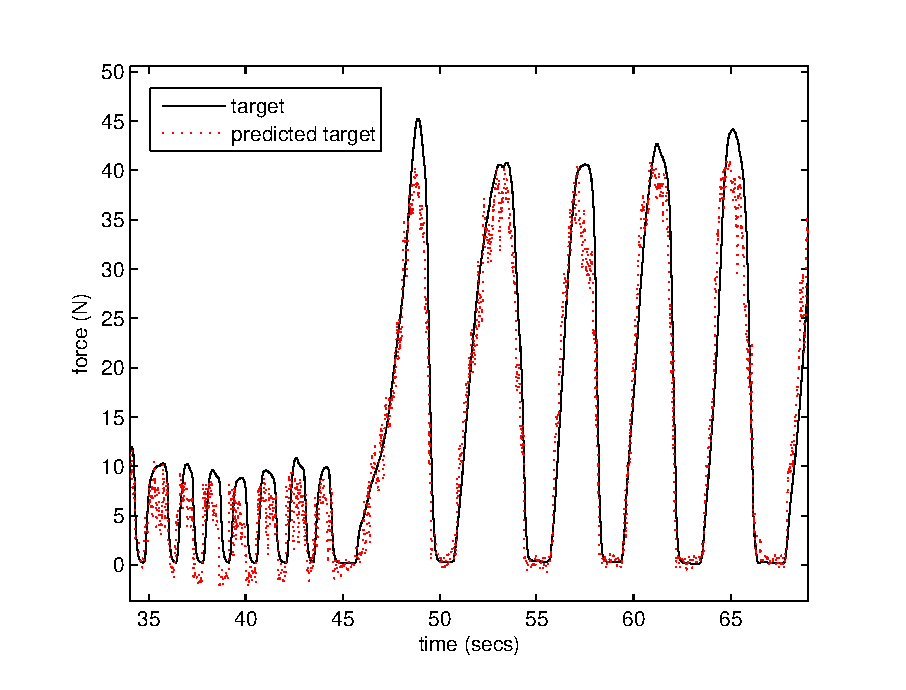
\includegraphics[width=0.30\textwidth]{figs/fig_regression1} &
    \includegraphics[width=0.30\textwidth]{figs/fig_regression2} &
    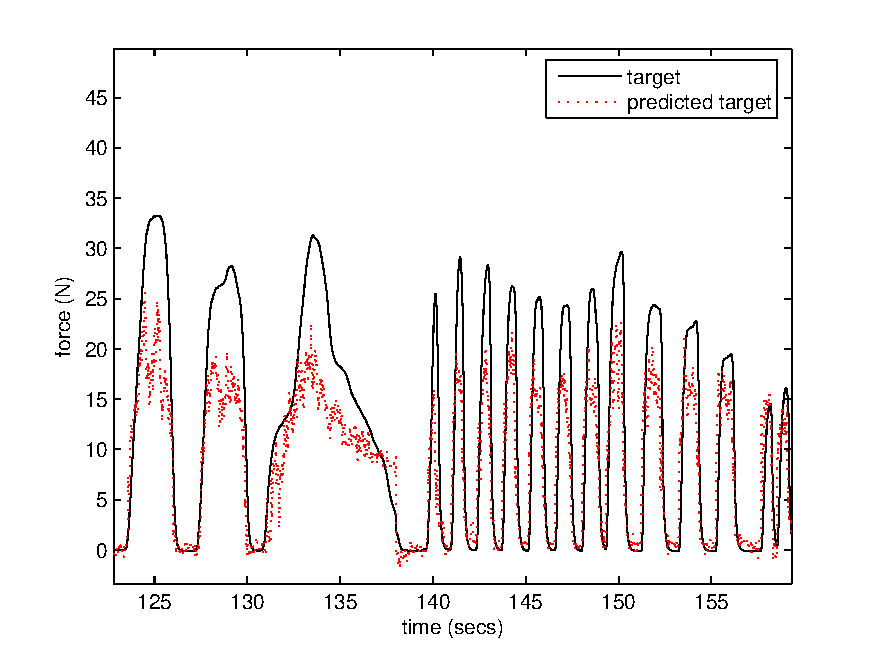
\includegraphics[width=0.30\textwidth]{figs/fig_regression3} \\
    session $6$, day $1$ & session $10$, day $2$ & session $7$, day $1$ \\
    MSE: $4.85\cdot 10^4$ & MSE: $5.48\cdot 10^4$ & MSE: $10.21\cdot 10^4$ \\
  \end{tabular}
  \caption{Examples of real and predicted force target values.}
  \label{fig:regression}
\end{figure*}

A remarkable point in the Figure is the presence of a ``plateau''
effect, especially in the test with the worst performance, namely
session $7$ of day $1$ (third pane). As is apparent, the predicted
target are mostly wrong in amplitude, being systematically
\emph{lower} than the correct values. Again, this is most likely due
to insufficient sampling in the region of interest.
